% !TeX program = pdflatex
% !BIB program = biber


\section{Introduction}
\label{sec:introduction}

Over the past recent years, technological advances have led to a remarkable increase in data collection capabilities and database sizes (\cite{wang2019information}). Datasets with hundreds of features or thousands to millions of instances are now common across many research fields and industries (\cite{li2013statistical}). From an economic research perspective, \textcite{einav2014data} emphasize the use of large administrative datasets to create innovative research designs and predictive models that may be challenging or infeasible to develop with smaller sample sizes or larger data aggregation. \\

However, even though massive data brings new opportunities for understanding different phenomena through rich datasets, its enormous volume also imposes large computational and statistical challenges (\cite{fan2014challenges}). For instance, conducting optimal estimation of parameters and inference could become cumbersome when dealing with a massive amount of information (\cite{ng2017opportunities}). The computational cost could be too high, or it might even become computationally infeasible to fit standard statistical models when the datasets are huge (\cite{han2020local}). \\

One common approach is to downsize the data volume by subsampling data points and fitting the methods in a much smaller sample, thus reducing computational burden while still being able to make statistical inferences about the full sample parameters (\cite{yu2023}). Since the variance of the estimates will be larger in smaller samples, there is an inevitable trade-off between statistical efficiency and computational gains, and designing an effective subsampling scheme that reduces this trade-off becomes crucial (\cite{lee2020economics}, \cite{han2020local}). However, for imbalanced datasets, where the target variable shows a significantly unequal distribution between the classes, subsampling becomes more of a challenge  (\cite{he2019}). The most naive approach, uniform subsampling, will most likely fail to construct meaningful samples, as it assigns the same acceptance probability to each data point (\cite{hastie2014}, \cite{han2020local}, \cite{wang2020rare}, \cite{yao2021review}, \cite{cheng2020}).\\

First originated in epidemiology, case-control is a well-known subsampling design mostly used in medical research to assess risk factors related to rare diseases (\cite{rose2008}). It improves upon uniform subsampling by having different acceptance probabilities for ``cases'' (minority class) and ``controls'' (majority class). A logistic regression is then fitted to the subsample, and estimates of the population parameters are retrieved after making an adjustment to the intercept. The case-control estimate is asymptotically consistent and unbiased in scenarios when there is high marginal imbalance, and the model is correctly specified. Additionally, weighted case-control estimate has been proven to be efficient under model misspecification and mild marginal imbalance (\cite{prentice1979}, \cite{king2001logistic}, \cite{scott1986}, \cite{shen2021surprise}). More recently, \textcite{hastie2014} proposed a local-case control subsampling design that aims to improve upon standard case-control methods by balancing the classes locally in the feature space via an accept–reject subsampling scheme. Their method is consistent even under misspecification, and it is argued to exploit the conditional imbalance in the data.

% Two types of imbalance have been identified in the relevant literature: marginal imbalance and conditional imbalance (\cite{hastie2014}, \cite{obrien2019}, \cite{han2020local}). The former refers to the case when one of the classes is rare throughout the feature space, while the latter considers the situation when one class is predominant for a subset of the feature space but rare for the rest of the feature space (\cite{obrien2019}). 

 

\begin{figure}[ht]
  \centering
    \scalebox{0.4}{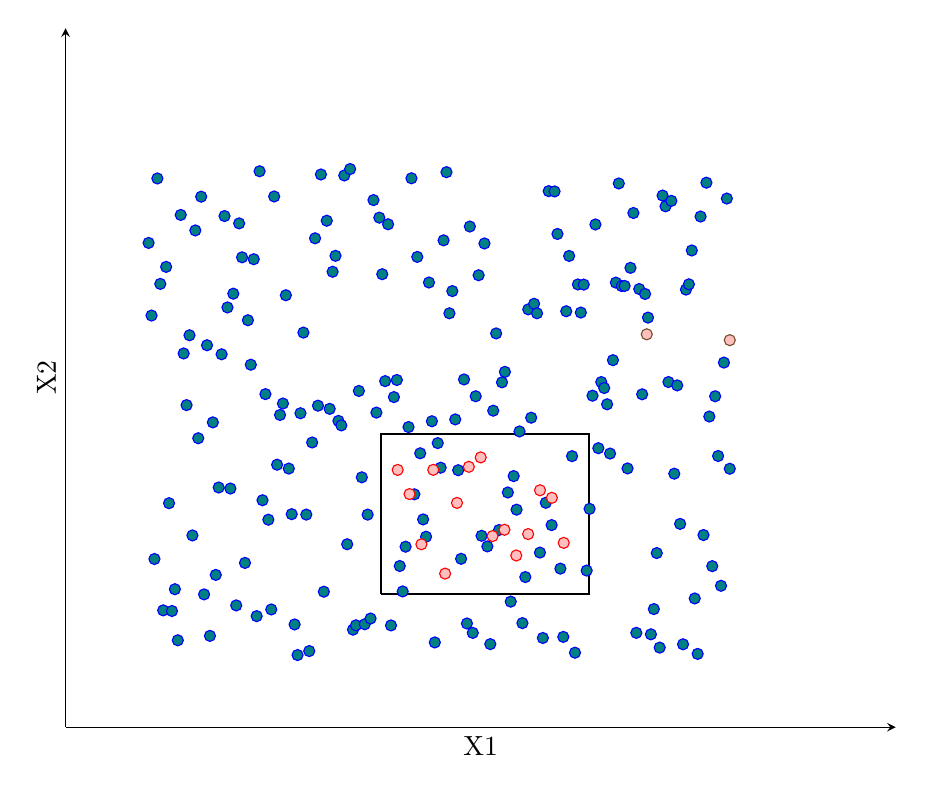
\begin{tikzpicture}
  \begin{axis}[
        width=\linewidth,
        xmin=0,xmax=10,ymin=0,ymax=100, 
        xlabel=X1,
        ylabel=X2,
        ticks=none,
        axis x line=bottom,axis y line=left
        ]
       \addplot+[y filter/.expression={y+10},only marks,mark=*, mark options = {fill=teal},samples=200,domain=1:8] {70*rnd};
       \addplot+[y filter/.expression={y+20},only marks,mark=*,mark options={fill=pink},samples=15,domain=4:6] {20*rnd};
      \addplot+[y filter/.expression={y+50},only marks,mark=*,mark options={fill=pink},samples=2,domain=7:8] {20*rnd};
       \draw[thick] (3.8, 19) -- (6.3,19) -- (6.3,42) -- (3.8, 42) -- (3.8, 19);
  \end{axis}
\end{tikzpicture}}
    \caption[Graphical example of the between-class imbalance problem.]{A two-dimensional graphical representation of a between-class imbalance problem based on \cite{he2019}. The blue instances represent the majority class, while the pink observations the minority class.}
    \label{fig:imbalance}
\end{figure}

The aim of this thesis is to study the statistical performance of the three above-mentioned case-control methods in approximating the true population parameters. Section \ref{sec:Methods} shows the estimation of the Maximum Likelihood logistic regression estimate and discusses how large samples could affect its computation. Section \ref{sec:subsampling} introduces the subsampling algorithms under study and shows their underlying statistical assumptions for consistency and unbiasedness. Section \ref{sec:metrics} presents the metrics for evaluating the methods. Section \ref{sec:sim_study} contains the numerical exercises conducted to compare the performance of the methods across different levels of marginal imbalance and sample sizes. It also shows an empirical analysis of the asymptotic properties of the local-case control, focusing on the assumption of a data-independent pilot for approximating its asymptotic distribution. Section \ref{sec:data} illustrates the performance of the methods in a real dataset, and Section \ref{sec:Conclusion} concludes.

% Their statistical properties and assumptions are examined in both a simulation study and a real-world imbalanced dataset.
